\section{Self-play}

Le self-play démarre le 7 avril à 00 h 34, à partir du checkpoint de
l'affinage converti au format du self-play
(\chemin{convert\_ckpt.py}, sortie
\chemin{2026\_04\_07\_00h10\_UNSUPERVISED\_NEW\_MODEL.pt}).

\subsection{La recette}

\begin{itemize}[leftmargin=1.2em,itemsep=2pt,topsep=2pt]
  \item \textbf{Parties} : 512 par itération, sauf les itérations 27 à 37
        (256 par itération, pendant la transition vers le self-play batché
        sur GPU).
  \item \textbf{Recherche} : MCTS, 700 simulations sur les coups lents et
        100 sur les coups rapides, avec 25 \% de coups lents. Table de
        transposition de 4 millions d'entrées. Génération des parties en C++
        avec inférence batchée sur GPU à partir du 13 avril.
  \item \textbf{Entraînement} : AdamW ($\text{weight decay} = 10^{-4}$),
        learning rate $5 \cdot 10^{-6}$ au premier run, puis $5 \cdot 10^{-5}$,
        $2 \cdot 10^{-5}$ et $4 \cdot 10^{-5}$ à partir du 14 avril. Lot de
        2\,048 puis 4\,096, précision mixte 16 bits.
  \item \textbf{Buffer} : 750\,000 positions sur disque, en shards. Chaque
        itération échantillonne 14 fois le volume de positions qu'elle vient
        de générer.
  \item \textbf{Évaluation} : 16 parties contre Stockfish limité à
        200\,000 nœuds toutes les 8 itérations, avec une ancre montée de
        2\,200 à 2\,300, 2\,450 puis 2\,600 Elo.
\end{itemize}

\subsection{Déroulé et volumes}

Les 436 itérations se répartissent sur 26 lancements, chacun reprenant le
checkpoint du précédent (annexe~A). Au total : 211\,200 parties générées,
5,93 M de positions conservées pour l'entraînement, 21,7 M de coups joués et
26\,356 steps d'optimiseur, soit 105,9 M d'échantillons vus.

\begin{figure}[h]
\centering
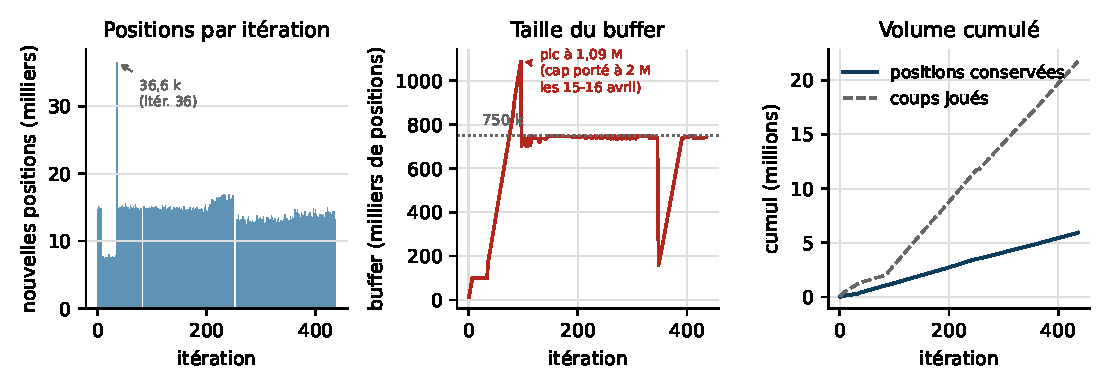
\includegraphics[width=\textwidth]{figures/fig_selfplay_volume.pdf}
\caption{Volume du self-play. À gauche, les positions générées par itération
(le pic de l'itération 36 vient d'un lancement qui en a conservé davantage).
Au centre, la taille du buffer, avec un pic à 1,09 M quand le plafond a été
porté temporairement à 2 M les 15 et 16 avril. À droite, les cumuls : les
positions conservées (coups lents) et l'ensemble des coups joués.}
\label{fig:volume-selfplay}
\end{figure}

Le rapport entre les deux courbes du panneau de droite est cohérent avec la
recette : seuls les coups joués sous recherche lente sont conservés comme
positions d'entraînement, soit environ un quart des coups. Le buffer, lui,
reste plein à 750\,000 positions : le modèle ne réapprend donc jamais deux
fois le même échantillon, il tourne sur ses parties les plus récentes.

\subsection{Pertes et learning rate}

\begin{figure}[h]
\centering
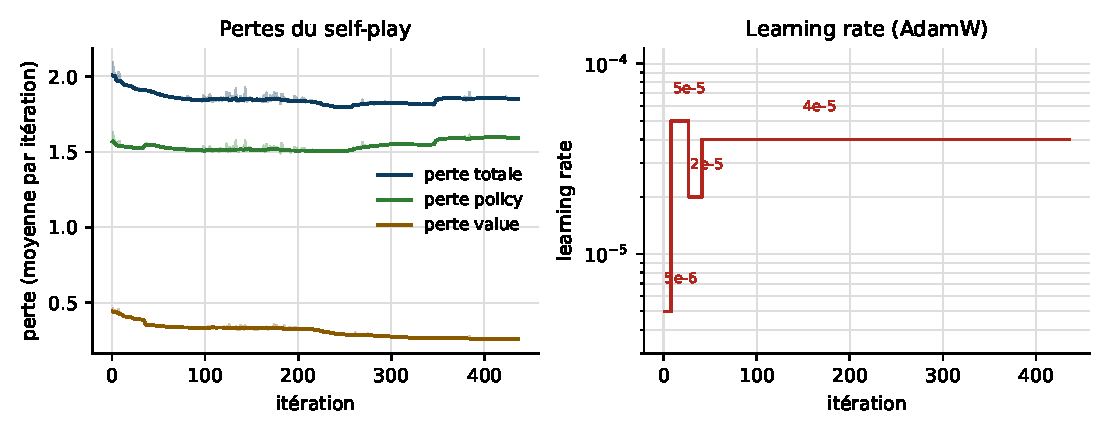
\includegraphics[width=\textwidth]{figures/fig_selfplay_pertes.pdf}
\caption{À gauche, les pertes du self-play, valeurs brutes (traits fins) et
médiane glissante sur 21 itérations (traits épais). À droite, l'évolution du
learning rate.}
\label{fig:pertes-selfplay}
\end{figure}

La perte totale passe d'environ 1,94 à 1,86 en médiane. La perte value, elle,
baisse nettement, d'environ 0,41 à 0,26 : le modèle devient sensiblement
meilleur pour prédire le résultat des positions. La perte policy reste
autour de 1,54 à 1,60, avec une légère remontée.

\begin{attention}
La perte policy du self-play n'est pas comparable d'une itération à l'autre :
la cible est la politique de recherche du modèle lui-même et le jeu de
données glisse en permanence. Une remontée de cette courbe ne signifie pas
une régression, c'est aussi le signe que les positions deviennent plus
difficiles. La perte value, ancrée sur le résultat réel des parties, est le
meilleur indicateur de progression de cette phase.
\end{attention}

\subsection{Qualité des parties}

\begin{figure}[h]
\centering
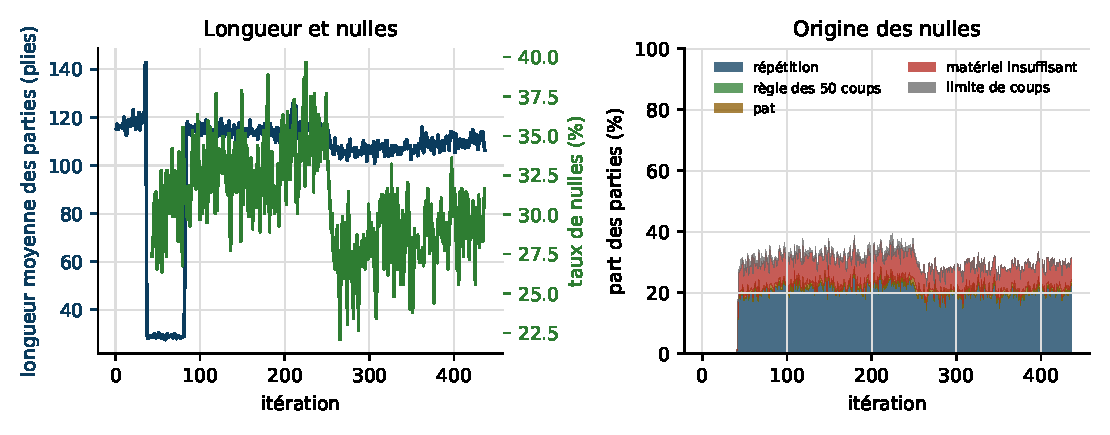
\includegraphics[width=\textwidth]{figures/fig_selfplay_qualite.pdf}
\caption{À gauche, la longueur moyenne des parties (en plies) et le taux de
nulles. À droite, la décomposition des nulles par cause.}
\label{fig:qualite-selfplay}
\end{figure}

Les parties durent environ 117 plies au début, puis se stabilisent autour de
105 à 110 plies. Le taux de nulles reste autour de 30 \%, dominé par les
répétitions (environ 20 \% des parties) et le matériel insuffisant (environ
8 \%). La règle des 50 coups, le pat et la limite de coups restent marginaux.
Les pics de nulles par répétition autour des itérations 60 à 100
correspondent aux périodes où le tirage de Dirichlet et la température
favorisaient l'exploration.

\subsection{Niveau face à Stockfish}

\begin{figure}[h]
\centering
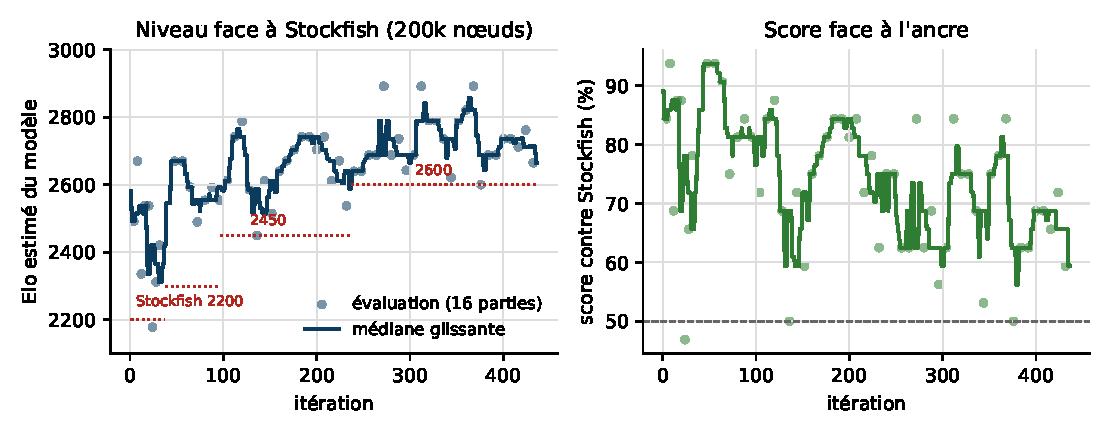
\includegraphics[width=\textwidth]{figures/fig_elo.pdf}
\caption{Niveau estimé face à Stockfish, 200\,000 nœuds et 16 parties par
évaluation. La ligne pointillée rouge indique l'Elo de l'ancre, qui change
en cours de route : les estimations ne sont donc pas sur la même échelle
d'une période à l'autre. À droite, le score brut contre l'ancre.}
\label{fig:elo}
\end{figure}

La première évaluation, à l'itération 4, donne 2\,492 Elo. La dernière, à
l'itération 432, donne 2\,665 Elo ; le maximum observé est 2\,892. La série
est très bruitée : chaque point ne repose que sur 16 parties, ce qui donne
une incertitude de l'ordre de $\pm 150$ Elo. Les paliers visibles dans le
score (60, 75, 85 \%) suivent surtout les changements d'ancre, et non des
sauts de niveau du modèle. La tendance de fond reste une progression claire
entre le début du self-play (autour de 2\,490) et la fin (autour de 2\,650),
avec des passages réguliers au-dessus de 2\,750.
